% SIGIR Resources Track (ACM sigconf) LaTeX template scaffold
% -------------------------------------------------------------------
% This is a lightweight ACM 'acmart' (sigconf) project intended for:
% (1) migrating an existing draft into the SIGIR format, and
% (2) iterating section-by-section without breaking compilation.
%
% Notes on anonymity:
% - SIGIR 2026 Resources Track is single-anonymous (author names listed).
% - Do NOT enable anonymous mode; fill in the real author list below.

\documentclass[sigconf,natbib=true,review]{acmart}
% \documentclass[sigconf,natbib=true,review,anonymous=true]{acmart}

% For camera-ready (typically):
% \documentclass[sigconf,natbib=true]{acmart}

% Many conferences request suppressing ACM rights / ref-format blocks for review.
\setcopyright{none}
\settopmatter{printacmref=false} % hide ACM Reference Format block
\renewcommand\footnotetextcopyrightpermission[1]{}

\usepackage{booktabs}
\usepackage{multirow}
\usepackage{amsmath}
% acmart already loads a math font package that conflicts with amssymb's \Bbbk.
% Keep the dependency set minimal to avoid symbol redefinition errors.
% \usepackage{amssymb}
\usepackage{mathtools}
\usepackage{enumitem}
\usepackage{url}

% Figures / diagrams
\usepackage{graphicx}
\usepackage{tikz}
\usetikzlibrary{positioning,arrows.meta}

% Algorithms (used in the migrated draft)
\usepackage{algorithm}
\usepackage{algpseudocode}

% Optional: algorithms (uncomment if you used them in the draft)
% \usepackage{algorithm}
% \usepackage{algpseudocode}

\title[EdgeQA]{EdgeQA: Model-Aware Synthesis of Unknown and Brittle Knowledge Questions from Unlabeled Text with Knowledge Coverage Evaluation}

% -------------------------------------------------------------------
% Authors
% Replace with your real author list for single-blind tracks.
% For double-anonymous, keep only '\author{Anonymous}' and remove affiliations.

% Single-anonymous submission: list real authors.
\author{Yuli Zhang}
\affiliation{%
  \institution{Beijing University of Posts and Telecommunications}
  \city{Beijing}
  \country{China}
}
\email{zhangyuli@bupt.edu.cn}

\renewcommand{\shortauthors}{Zhang}

% -------------------------------------------------------------------
\begin{abstract}
Large language models (LLMs) perform well on many knowledge-intensive tasks, yet they remain unreliable in domains where their parametric knowledge is incomplete, long-tailed, or compositionally expressed.
Existing synthetic question--answer (QA) pipelines largely optimize for scale or downstream fine-tuning gains, often producing questions whose answers are already known to the target model and offering limited diagnostics of how well a synthetic QA set represents the underlying corpus.
We present \textbf{EdgeQA}, an \emph{API-only}, model-aware pipeline that converts unlabeled corpora into evidence-grounded QA pairs \emph{targeting unknown and brittle knowledge of a specified target model}.
EdgeQA mines knowledge-rich passages, generates candidates with minimal evidence spans, scores unknownness and brittleness via closed-book failure and inconsistency signals (sampling and paraphrases), filters for grounding and ambiguity, and selects a budgeted subset to maximize \emph{document}, \emph{knowledge-unit}, and \emph{reasoning-type} coverage.
We additionally introduce \textbf{EdgeCoverBench}, a coverage-aware stress-test benchmark with paraphrases, near-miss counterfactuals, and unanswerable items to evaluate robustness and abstention.
In this resource release, we instantiate EdgeQA on two CC-BY textbooks (Open Logic Project; OpenStax University Physics), export BEIR-style retrieval test collections (queries/corpus/qrels), and provide a coverage-and-cost evaluation suite with token-budget curves under \textsc{DeepSeek-V3.2} (\texttt{deepseek-chat} / \texttt{deepseek-reasoner}) settings.
\end{abstract}

\keywords{information retrieval, evaluation, datasets, large language models, question answering}

% If you include CCS concepts, uncomment and fill these in.
% \begin{CCSXML}
% <ccs2012>
%  <concept>
%   <concept_id>10010147.10010257</concept_id>
%   <concept_desc>Computing methodologies~Information extraction</concept_desc>
%   <concept_significance>500</concept_significance>
%  </concept>
% </ccs2012>
% \end{CCSXML}
% \ccsdesc[500]{Computing methodologies~Information extraction}

\begin{document}

\maketitle

\section{Introduction}
\label{sec:intro}

Pretrained language models can store and recall relational knowledge present in their training data, enabling factual question answering without explicit retrieval~\citep{petroni2019lama}.
However, strong average performance masks systematic failures on domain-specific knowledge and long-tail facts, where relying on parametric memory alone is insufficient~\citep{mallen2023popqa}.
In practice, teams adapt LLMs to new domains either by collecting QA/instruction data for supervised fine-tuning (SFT) or by introducing retrieval-augmented generation (RAG).
When labeled data are scarce but a domain corpus is available, synthetic QA generation from unlabeled text becomes an attractive alternative.

Large-scale synthetic QA resources demonstrate that automated QA construction is feasible at scale.
PAQ~\citep{lewis2021paq} creates 65M ``probably asked'' QA pairs from Wikipedia to increase coverage and improve QA systems.
Benchmarks such as KILT~\citep{petroni2021kilt} unify knowledge-intensive tasks under a shared evidence source and evaluate provenance.
Yet, these frameworks do not directly answer a crucial question for \emph{model-targeted} domain adaptation and evaluation:
\emph{given a target model $M$ and a domain corpus $\mathcal{C}$, what subset of corpus knowledge is \textbf{unknown} or \textbf{brittle} for $M$, and how can we systematically build a QA resource that targets such edge knowledge while offering measurable \textbf{coverage} over $\mathcal{C}$ under a clear token/cost budget?}

Two observations motivate a model-aware construction approach.
First, LLMs can be inconsistent under meaning-preserving paraphrases, even for factual queries~\citep{elazar2021pararel}, and paraphrastic variability can substantially affect reasoning performance~\citep{srikanth2024paraphrastic}.
Second, black-box LLM APIs are increasingly used in RAG systems, but their behavior can vary with decoding, safety layers, and interface updates.
Together, these suggest that ``unknownness'' should be defined behaviorally (failure/instability), and that resources should report \textbf{coverage--budget curves} rather than only downstream fine-tuning gains.

\paragraph{IR interface: turning grounded QA into retrieval test collections.}
From an information retrieval perspective, each grounded QA instance naturally defines a \emph{query} (the question) and \emph{relevant documents} (the evidence passages).
Therefore, an EdgeQA dataset can be exported as a BEIR-style test collection (\texttt{queries.jsonl}, \texttt{corpus.jsonl}, \texttt{qrels})~\citep{thakur2021beir} and used to benchmark sparse, dense, and hybrid retrievers, as well as end-to-end RAG pipelines.
We treat this ``IR-ification'' as a first-class part of the resource release.

\paragraph{Resource overview.}
This paper describes a coverage-aware resource family consisting of:
(1) \textbf{EdgeQA}, a model-aware pipeline that converts unlabeled corpora into grounded QA pairs targeting unknown and brittle knowledge of a specified target model, and
(2) \textbf{EdgeCoverBench}, a corpus-based stress-test benchmark that operationalizes coverage via knowledge units and evaluates robustness under paraphrases, near-miss counterfactuals, and unanswerable items.
We additionally provide a \textbf{knowledge coverage evaluation protocol} that measures document coverage, knowledge-unit coverage, and reasoning-type coverage.

\begin{table}[t]
\centering
\small
\begin{tabular}{@{}p{2.2cm}p{6.2cm}p{1.4cm}@{}}
\toprule
\textbf{Artifact} & \textbf{What it provides} & \textbf{Sec.} \\\midrule
EdgeQA builder & End-to-end pipeline (ingest$\rightarrow$mine$\rightarrow$generate$\rightarrow$score/filter$\rightarrow$unit extract$\rightarrow$budgeted selection) for producing grounded QA resources from an unlabeled corpus for a target model $M$ & \S\ref{sec:edgeqa} \\
Coverage evaluation toolkit & Metrics and reporting protocol for DocCov / UnitCov / ReasonCov, unknownness purity, brittleness, and \emph{cost-aware} coverage curves & \S\ref{sec:edgeqa} \\
IR test collection export & BEIR-style export (queries/corpus/qrels) plus retriever baselines for each EdgeQA instantiation & \S\ref{sec:experiments} \\
EdgeCoverBench & Coverage-aware stress-test benchmark with canonical, paraphrase, near-miss, and unanswerable items; supports abstention and risk--coverage evaluation & \S\ref{sec:edgecoverbench} \\
\bottomrule
\end{tabular}
\caption{Summary of the resources described in this paper. Release links and licenses are specified in Sec.~\ref{sec:availability}.}
\label{tab:resource_summary}
\end{table}

\paragraph{Our goal.}
Given an unlabeled corpus $\mathcal{C}$ and a target model $M$, we construct a grounded QA set $\mathcal{Q}$ such that:
(i) $\mathcal{Q}$ targets \emph{unknown or brittle} knowledge for $M$ in closed-book mode,
(ii) each QA is \emph{answerable and grounded} in evidence from $\mathcal{C}$,
(iii) $\mathcal{Q}$ maximizes \emph{knowledge coverage} of $\mathcal{C}$ under a budget, and
(iv) $\mathcal{Q}$ covers diverse reasoning operators.

\paragraph{Contributions.}
\begin{enumerate}[leftmargin=*]
  \item We present \textbf{EdgeQA}, a pipeline for \emph{model-aware} synthetic QA generation that prioritizes unknown/brittle knowledge and selects a budgeted subset to maximize corpus coverage.
  \item We introduce a \textbf{coverage evaluation protocol} for QA sets, measuring document coverage, knowledge-unit coverage, and reasoning-type coverage alongside unknownness purity and brittleness.
  \item We describe \textbf{EdgeCoverBench}, a benchmark for robustness and abstention under unit-anchored coverage accounting.
  \item We export each instantiation as a \textbf{retrieval test collection} in BEIR format~\citep{thakur2021beir} and provide sparse/dense retrieval baselines, enabling IR- and RAG-centric reuse.
\end{enumerate}

\section{Related Work}
\label{sec:related}

\paragraph{Synthetic QA generation from unlabeled text.}
Automated QA construction has been explored for data scaling and downstream gains.
PAQ~\citep{lewis2021paq} generates ``probably asked'' questions to expand coverage relative to open-domain QA benchmarks such as Natural Questions~\citep{kwiatkowski2019naturalquestions} and SQuAD~2.0~\citep{rajpurkar2018squad2}.
In contrast, EdgeQA explicitly conditions selection on a specified target model's unknownness and brittleness, and evaluates the resulting QA set via \emph{corpus coverage under budget} rather than only supervised fine-tuning gains.

\paragraph{Knowledge probing and knowledge-intensive benchmarks with evidence.}
LAMA~\citep{petroni2019lama} probes factual relations in pretrained models, while KILT~\citep{petroni2021kilt} unifies knowledge-intensive tasks under a shared evidence source and evaluates provenance.
Our work is complementary: instead of evaluating model knowledge on a fixed benchmark, we \emph{construct} a benchmark from an arbitrary domain corpus and quantify how well it covers that corpus.

\paragraph{Retrieval test collections and reusable IR benchmarks.}
IR research relies on test collections with queries, corpora, and relevance judgments.
BEIR~\citep{thakur2021beir} standardized a heterogeneous format for evaluating sparse and dense retrieval models across many datasets.
Toolkits such as Pyserini~\citep{lin2021pyserini} further improve reproducibility by providing standardized sparse and dense retrieval pipelines.
Because each grounded QA instance provides a natural query (question) and relevance signals (evidence passages), EdgeQA can be exported as a BEIR-style collection and used to benchmark BM25~\citep{robertson2009bm25}, dense retrieval (e.g., DPR~\citep{karpukhin2020dpr}, sentence-BERT~\citep{reimers2019sentencebert}), and interaction-based retrievers (e.g., ColBERT~\citep{khattab2020colbert}).

\paragraph{RAG and parametric vs. non-parametric memory.}
Retrieval-augmented QA and generation couples retrieval with a reader or generator to improve factuality and robustness~\citep{chen2017drqa,guu2020realm,lewis2020rag,izacard2021fid}.
PopQA highlights that retrieval can outperform parametric memory on the long tail~\citep{mallen2023popqa}.
EdgeQA generalizes this insight by searching for \emph{model-specific} unknownness signals, which may correlate with but are not identical to corpus rarity.

\paragraph{Consistency, uncertainty, and self-knowledge.}
Behavioral testing frameworks such as CheckList~\citep{ribeiro2020checklist} and contrast sets~\citep{gardner2020contrastsets} emphasize robustness under minimal, meaning-preserving perturbations.
ParaRel~\citep{elazar2021pararel} reveals inconsistency of factual knowledge under paraphrased prompts.
For reasoning tasks, paraphrastic variability can account for a significant portion of performance variance, and the PC metric quantifies paraphrastic consistency~\citep{srikanth2024paraphrastic}.
Uncertainty calibration in black-box LLMs can be derived from sample consistency~\citep{lyu2024sampleconsistency}, and conformal methods can provide correctness coverage guarantees for uncertainty sets~\citep{wang2024conu}.
SelfAware evaluates whether models know what they do not know via unanswerable questions~\citep{yin2023selfaware}.
Risk--coverage analysis under abstention is closely related to selective classification~\citep{geifman2017selective}.
EdgeQA leverages these ideas to detect unknown/brittle knowledge and to build stress tests that measure robustness and abstention.

\paragraph{Grounding, attribution, and factuality.}
Hallucination and factuality diagnostics for LLMs include TruthfulQA~\citep{lin2022truthfulqa} and black-box self-consistency checks such as SelfCheckGPT~\citep{manakul2023selfcheckgpt}.
Attribution and factuality research emphasizes verifying support for generated content.
RARR performs post-hoc research and revision to retrofit attribution~\citep{gao2023rarr}.
FActScore decomposes generations into atomic facts and verifies support~\citep{min2023factscore}.
EdgeQA adopts similar principles to filter QA for answerability and grounding, and to define atomic-fact coverage units when deterministic structure is unavailable.

\paragraph{Knowledge coverage evaluation.}
Recent work evaluates medical knowledge coverage of LLMs using KGs, reporting entity/relation/triple-level coverage~\citep{zhang2025medkgeval}.
We generalize coverage from structured KGs to arbitrary unlabeled corpora, integrate coverage into dataset selection, and expose cost--coverage trade-offs for API-based construction.

\section{EdgeQA: Model-Aware QA Resource Construction}
\label{sec:edgeqa}

\subsection{Problem setup}
Let $\mathcal{C}=\{d_i\}_{i=1}^D$ be an unlabeled corpus, segmented into passages $\mathcal{P}=\{p_j\}_{j=1}^P$ (e.g., paragraphs).
A QA instance is $q=(x,y,E,t)$, where $x$ is the question, $y$ is the answer, $E\subseteq\mathcal{P}$ is the evidence set (one or more passages), and $t$ is a reasoning/operator label.
Given a target model $M$ (black-box API), we seek a QA set $\mathcal{Q}=\{q_k\}_{k=1}^N$ that satisfies:
\begin{enumerate}[leftmargin=*]
  \item \textbf{Grounding:} $y$ is supported/entailed by $E$.
  \item \textbf{Edge knowledge:} $x$ targets unknown/brittle knowledge for $M$ in closed-book mode.
  \item \textbf{Coverage:} $\mathcal{Q}$ spans $\mathcal{C}$ broadly under a budget.
\end{enumerate}

\subsection{Inputs, outputs, and record schema}
EdgeQA takes as input an unlabeled corpus $\mathcal{C}$, a target model $M$, and user-set budgets (candidate passage budget, generation budget, and final QA budget $N$).
It outputs a JSONL-style dataset where each example stores the QA pair, evidence mapping back into the corpus, and metadata required for coverage accounting and evaluation.
Table~\ref{tab:record_schema} summarizes a practical record schema.

\begin{table}[t]
\centering
\small
\begin{tabular}{@{}p{2.9cm}p{6.7cm}@{}}
\toprule
\textbf{Field} & \textbf{Description} \\\midrule
\texttt{question} & Question text $x$ \\
\texttt{answer} & Reference answer $y$ (short, grounded) \\
\texttt{evidence} & List of evidence items (doc/passage ids and offsets); supports rehydration from the raw corpus \\
\texttt{evidence\_span} & Minimal supporting span (character offsets or sentence indices) \\
\texttt{reason\_type} & Reasoning/operator label $t$ (manual or classifier) \\
\texttt{units} & Knowledge-unit ids covered by this QA (KG triples / atomic facts / structured units) \\
\texttt{scores} & Edge signals (closed-book correctness, sampling entropy, paraphrase agreement, verifier score) \\
\texttt{filters} & Filter decisions (groundedness, ambiguity, near-duplicate, copy/triviality) \\
\bottomrule
\end{tabular}
\caption{Suggested EdgeQA example schema (fields can be omitted when unavailable).}
\label{tab:record_schema}
\end{table}

\subsection{Pipeline overview}
Figure~\ref{fig:pipeline} summarizes the pipeline.
EdgeQA comprises (i) knowledge-rich passage mining, (ii) candidate QA generation, (iii) model-aware edge scoring, (iv) grounding and quality filtering, and (v) coverage-aware budgeted selection.

\begin{figure}[t]
\centering
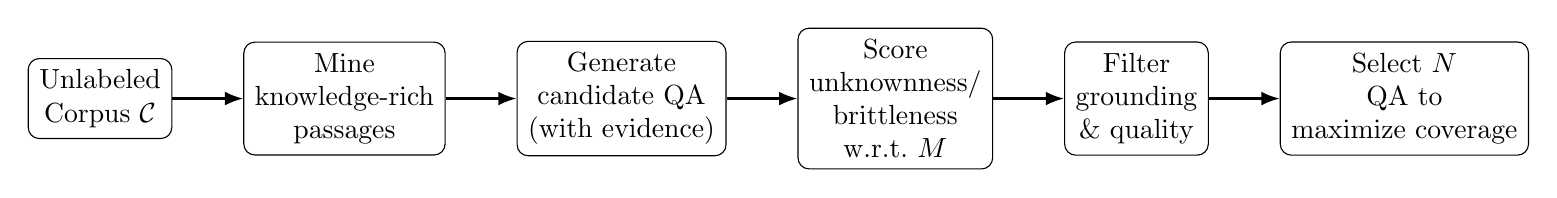
\begin{tikzpicture}[
  box/.style={draw, rounded corners, align=center, inner sep=4pt},
  arrow/.style={-Latex, thick},
  node distance=0.8cm and 0.9cm
]
\node[box] (corp) {Unlabeled\\Corpus $\mathcal{C}$};
\node[box, right=of corp] (mine) {Mine\\knowledge-rich\\passages};
\node[box, right=of mine] (gen) {Generate\\candidate QA\\(with evidence)};
\node[box, right=of gen] (score) {Score\\unknownness/\\brittleness\\w.r.t.\ $M$};
\node[box, right=of score] (filter) {Filter\\grounding\\\& quality};
\node[box, right=of filter] (select) {Select $N$\\QA to\\maximize coverage};
\draw[arrow] (corp) -- (mine);
\draw[arrow] (mine) -- (gen);
\draw[arrow] (gen) -- (score);
\draw[arrow] (score) -- (filter);
\draw[arrow] (filter) -- (select);
\end{tikzpicture}
\caption{EdgeQA pipeline: corpus $\rightarrow$ model-aware edge scoring $\rightarrow$ grounding filtering $\rightarrow$ coverage-aware selection.}
\label{fig:pipeline}
\end{figure}

\subsection{Knowledge-rich passage mining}
We prioritize passages likely to contain query-worthy domain knowledge.
We compute a salience score $s(p)$ with interpretable features (entity density, definitional cues, numeric constraints, term rarity) and optionally a topic coverage component to avoid topical collapse:
\begin{equation}
s(p) = \alpha\,\textsc{EntityDen}(p) + \beta\,\textsc{RelCue}(p) + \gamma\,\textsc{Rarity}(p) + \delta\,\textsc{TopicRep}(p).
\end{equation}
We then select a candidate set $\mathcal{P}_0$ by top-$K$ scoring or stratified sampling across clusters.

\subsection{Candidate QA generation}
For each $p\in \mathcal{P}_0$, a generator model $G$ produces one or more QA candidates $(x,y)$ along with explicit evidence spans.
We support two generation modes:
\begin{enumerate}[leftmargin=*]
  \item \textbf{Single-hop:} $E=\{p\}$, answerable within one passage.
  \item \textbf{Multi-hop:} select an evidence chain $E=\{p^{(1)},p^{(2)}\}$ via entity overlap or similarity, then generate a question requiring joint evidence.
\end{enumerate}
To enable downstream coverage accounting, each candidate also includes evidence identifiers and optional reasoning-type labels.

\subsection{Model-aware edge scoring}
We define ``edge'' questions as those that are \emph{unknown} or \emph{brittle} for the target model $M$ in closed-book mode.
Our scoring uses multiple behavior-based signals.

\paragraph{Closed-book failure.}
Let $\hat{y}^{cb}=M(x)$ be the closed-book answer (no evidence).
Define $\textsc{CB}(x)=\mathbb{1}[\hat{y}^{cb}\approx y]$, where $\approx$ is exact match or judged semantic equivalence.

\paragraph{Sampling inconsistency.}
We sample $m$ outputs from $M$ for the same $x$ under stochastic decoding and compute semantic entropy over clustered answers:
\begin{equation}
H_s(x) = -\sum_{c\in \mathcal{C}(x)} p_c \log p_c,\quad p_c=\frac{|c|}{m}.
\end{equation}
This follows the idea that sample consistency provides a proxy for confidence in black-box LLMs~\citep{lyu2024sampleconsistency}.

\paragraph{Paraphrase inconsistency.}
We generate $k$ meaning-preserving paraphrases $\{x^{(i)}\}_{i=1}^k$ and obtain closed-book answers $\hat{y}^{(i)}=M(x^{(i)})$.
To reduce dependence on a single ``anchor'' answer, we measure pairwise agreement:
\begin{equation}
A_p(x)=\frac{2}{k(k-1)}\sum_{1\le i<j\le k} \mathbb{1}[\hat{y}^{(i)}\approx \hat{y}^{(j)}].
\end{equation}
Paraphrase inconsistency is substantial for factual probing~\citep{elazar2021pararel} and reasoning~\citep{srikanth2024paraphrastic}.

\paragraph{Evidence-based verification.}
Given evidence $E$, we obtain $\hat{y}^{ctx}=M(x\mid E)$ and a verifier score $V(x,y,E)\in[0,1]$ checking whether $y$ is supported by $E$.
Verification can be implemented via NLI-style entailment checks or LLM-based judging, inspired by attribution and factuality work~\citep{gao2023rarr,min2023factscore}.
In our design, $V$ is primarily used as a \emph{grounding filter} (Sec.~\ref{sec:filtering}), rather than as an ``edge-ness'' signal.

\paragraph{Unified edge score.}
We combine behavior-based signals into an edge score:
\begin{equation}
U(x) = w_1 (1-\textsc{CB}(x)) + w_2 H_s(x) + w_3(1-A_p(x)).
\label{eq:edge_score}
\end{equation}
We keep candidates with $U(x)\ge \tau$ and that pass grounding/quality filters.
As an optional extension, we can calibrate $\tau$ to control error rates using conformal prediction ideas for LLM uncertainty~\citep{wang2024conu}.

\subsection{Filtering for grounding, answerability, and ambiguity}
\label{sec:filtering}
Synthetic QA resources often fail due to weak grounding.
We apply multi-stage filtering:
\begin{enumerate}[leftmargin=*]
  \item \textbf{Answerability with evidence:} require $\hat{y}^{ctx}\approx y$ and/or $V(x,y,E)$ above a threshold.
  \item \textbf{Grounding:} require minimal supporting spans and agreement between $y$ and the evidence snippet.
  \item \textbf{Ambiguity:} remove questions with multiple plausible answers not disambiguated by $E$.
  \item \textbf{Trivial copy questions:} remove questions that overly copy the evidence (e.g., high lexical overlap between $x$ and the evidence span, or template-like extractive prompts).
\end{enumerate}

\subsection{Coverage-aware budgeted selection}
After filtering, we obtain a pool $\mathcal{Q}_{pool}$.
Given a final QA budget $N$, we select $\mathcal{Q}\subseteq\mathcal{Q}_{pool}$ to maximize coverage while penalizing redundancy:
\begin{equation}
\max_{|\mathcal{Q}|=N}\; F(\mathcal{Q})=
\lambda_d\,\textsc{DocCov}(\mathcal{Q})+\lambda_u\,\textsc{UnitCov}(\mathcal{Q})+\lambda_r\,\textsc{ReasonCov}(\mathcal{Q})
-\lambda_{dup}\,\textsc{Redundancy}(\mathcal{Q}).
\end{equation}
Coverage terms are set-coverage-like and often exhibit diminishing returns.
When $F$ is monotone submodular (e.g., pure set coverage), a greedy selector provides a $(1-1/e)$ approximation guarantee; in practice, greedy remains a scalable heuristic.

\paragraph{Unknownness-purity constraint (optional).}
Some applications require the selected set to contain at least a fraction $\rho$ of \emph{unknown} items (Sec.~\ref{sec:metrics_unknown_brittle}).
We support a simple proportion constraint, e.g.,
$\frac{1}{|\mathcal{Q}|}\sum_{q\in\mathcal{Q}}\mathbb{1}[q\text{ is unknown}]\ge\rho$, implemented by constrained greedy or two-pool selection.

\begin{algorithm}[t]
\caption{EdgeQA construction (high-level)}\label{alg:edgeqa}
\begin{algorithmic}[1]
\Require Corpus $\mathcal{C}$, target model $M$, generator $G$, budget $N$
\Ensure QA set $\mathcal{Q}$

\State Segment $\mathcal{C}$ into passages $\mathcal{P}$
\State Mine candidate passages $\mathcal{P}_0 \subseteq \mathcal{P}$ using salience $s(p)$
\State Initialize empty pool $\mathcal{Q}_{pool}\leftarrow \emptyset$
\For{each passage (or chain) $E$ from $\mathcal{P}_0$}
  \State Generate candidates $\{(x,y,t)\}$ from $G$ conditioned on $E$
  \For{each candidate $(x,y,t)$}
    \State Compute edge score $U(x)$ w.r.t.\ $M$ (closed-book, sampling, paraphrase)
    \If{$U(x)\ge\tau$ and passes grounding/ambiguity filters}
      \State Add $q=(x,y,E,t)$ to $\mathcal{Q}_{pool}$
    \EndIf
  \EndFor
\EndFor
\State Extract knowledge units $\mathcal{U}$ from $\mathcal{C}$ (Sec.~\ref{sec:unitcov})
\State Select $\mathcal{Q}\subseteq \mathcal{Q}_{pool}$, $|\mathcal{Q}|=N$ by greedy maximization of $F(\mathcal{Q})$
\State \Return $\mathcal{Q}$
\end{algorithmic}
\end{algorithm}

\subsection{Knowledge coverage evaluation protocol}
We evaluate QA sets as representations of corpus/domain knowledge, complementing task accuracy.
Table~\ref{tab:metrics} summarizes the proposed metrics.

\begin{table}[t]
\centering
\small
\begin{tabular}{@{}p{2.6cm}p{5.2cm}p{2.9cm}@{}}
\toprule
\textbf{Metric} & \textbf{What it measures} & \textbf{Implementation notes} \\\midrule
Document coverage & Fraction of passages exercised by at least one QA evidence set & Requires evidence mapping $E(q)$ \\
Knowledge-unit coverage & Fraction of extracted units (triples / atomic facts / structured units) covered by QA & Report multiple instantiations; analyze extractor noise \\
Reasoning-type coverage & Coverage/diversity over reasoning operators & Requires taxonomy and labeling \\
Unknownness purity & Closed-book failure but evidence-based success & Avoid circular judging; sample human audit \\
Brittleness rate & Sampling/paraphrase inconsistency & Report by reasoning type \\
Grounding pass rate & Verifier + human check on support & Use conservative thresholds \\
\bottomrule
\end{tabular}
\caption{Coverage and quality metrics for evaluating a synthetic QA set beyond SFT gains.}
\label{tab:metrics}
\end{table}

\subsubsection{Document-to-QA coverage}
Let $\mathcal{P}$ be all passages and $E(q)$ evidence passages for QA $q$.
\begin{equation}
\textsc{DocCov}(\mathcal{Q})=\frac{|\{p\in\mathcal{P}: \exists q\in\mathcal{Q},\, p\in E(q)\}|}{|\mathcal{P}|}.
\end{equation}
We additionally report coverage concentration (entropy) and marginal coverage curves as $|\mathcal{Q}|$ increases.

\subsubsection{Knowledge-unit coverage}
\label{sec:unitcov}
We use two instantiations and recommend reporting both.

\paragraph{KG-style units.}
Extract triples $(h,r,t)$ via OpenIE/relation extraction to define $\mathcal{U}_{KG}$.
Define $\textsc{UnitCov}_{KG}(\mathcal{Q})=\frac{|\cup_{q\in\mathcal{Q}}\textsc{Units}_{KG}(q)|}{|\mathcal{U}_{KG}|}$.
We also report entity-coverage and relation-coverage as diagnostics.

\paragraph{Atomic-fact units.}
Decompose passages into atomic facts, following factuality evaluation~\citep{min2023factscore}.
Let $\mathcal{U}_{AF}$ be the set of atomic facts and define $\textsc{UnitCov}_{AF}$ analogously.
To evaluate robustness, we recommend re-running unit extraction with different prompts/extractors and reporting coverage variance.

\paragraph{Structured units for expert corpora.}
Many expert corpora (math textbooks, statutes/regulations, and scientific guidelines) have strong intrinsic structure (e.g., Definition/Theorem/Article/Clause) that enables deterministic unit extraction.
When such structure is available, we recommend reporting structured-unit coverage alongside KG-style and atomic-fact coverage.

\subsubsection{Reasoning-type coverage}
\label{sec:reasoncov}
We define a reasoning taxonomy $\mathcal{T}$ and assign each QA a label $t(q)$ via a classifier and human audit.
Table~\ref{tab:reason} gives a minimal taxonomy we found practical for coverage reporting.

\begin{table}[t]
\centering
\small
\begin{tabular}{@{}p{2.6cm}p{7.7cm}@{}}
\toprule
\textbf{Type} & \textbf{Example operator / requirement} \\\midrule
Definition & ``What is X?'' grounded in definitional sentences \\
Attribute / relation & ``What property does X have?''; entity--attribute mapping \\
Comparison & ``Which is larger/earlier/more effective?''; pairwise compare \\
Temporal / causal & ordering, prerequisite, cause--effect statements \\
Numeric & arithmetic, threshold checks, unit conversion, count \\
Derivation / proof & symbolic manipulation; proof-step reasoning grounded in text \\
Multi-hop & requires combining evidence across $\ge 2$ passages \\
\bottomrule
\end{tabular}
\caption{A minimal reasoning taxonomy for reporting reasoning-type coverage.}
\label{tab:reason}
\end{table}

We report:
(i) $\textsc{ReasonCov}(\mathcal{Q})=\frac{|\{t(q):q\in\mathcal{Q}\}|}{|\mathcal{T}|}$ and
(ii) entropy over types as a diversity measure.
We additionally stratify brittleness (sampling entropy/paraphrase agreement) by $t$ to identify fragile operators.

\subsubsection{Unknownness and brittleness metrics}
\label{sec:metrics_unknown_brittle}
To avoid relying solely on downstream training gains, we directly measure:
\begin{align}
\textsc{UnknownPurity}(\mathcal{Q}) &= \frac{1}{|\mathcal{Q}|}\sum_{q\in\mathcal{Q}} \mathbb{1}[\textsc{CB}(x)=0 \wedge \textsc{CTX}(x,E)=1],\\
\textsc{BrittleRate}(\mathcal{Q}) &= \frac{1}{|\mathcal{Q}|}\sum_{q\in\mathcal{Q}} \mathbb{1}[H_s(x)\ge h \;\vee\; A_p(x)\le a],
\end{align}
where $\textsc{CTX}(x,E)=\mathbb{1}[\hat{y}^{ctx}\approx y]$, and $h,a$ are fixed thresholds or percentiles.

\paragraph{Implementation notes (draft).}
To facilitate reproducibility, we recommend reporting:
(i) passage segmentation policy,
(ii) candidate passage budget $|\mathcal{P}_0|$,
(iii) sampling settings ($m$ samples, temperature/top-$p$),
(iv) paraphrase settings ($k$ paraphrases and validation rules),
(v) answer equivalence function for $\approx$ (string match vs.\ judge model), and
(vi) verification model/prompt, threshold, and audited error rate.

% =========================
% EdgeCoverBench (revised for API-only construction)
% =========================

\section{EdgeCoverBench: Coverage-Aware Stress-Test Benchmark}
\label{sec:edgecoverbench}

\paragraph{Motivation.}
Standard QA benchmarks measure accuracy on a fixed question set, but they do not explicitly quantify (i) \emph{how much} of a domain corpus is exercised by the benchmark or (ii) the \emph{cost} required to reach a target coverage level when the benchmark is constructed via LLM APIs.
We introduce \textbf{EdgeCoverBench}, a corpus-based benchmark that operationalizes coverage via an explicit inventory of \textbf{knowledge units} and evaluates models with evidence-grounded questions, robustness tests, and abstention.

\paragraph{Release scope.}
To keep the resource self-contained and redistributable, this release instantiates EdgeCoverBench on the same two CC-BY corpora as EdgeQA (Sec.~\ref{sec:experiments}): the \textbf{Open Logic Project} (formal logic; LaTeX structure) and \textbf{OpenStax University Physics} (quantitative physics; textbook structure).
The benchmark design is general and can be applied to other structured domains, but we focus on these two for reproducible unit extraction and unambiguous evidence.

\subsection{Benchmark components}
EdgeCoverBench consists of:
\begin{enumerate}[leftmargin=*]
  \item a corpus snapshot $\mathcal{C}$ with stable passage identifiers and offsets,
  \item a unit inventory $\mathcal{U}$ extracted deterministically from document structure when available,
  \item unit-anchored QA instances with minimal evidence spans,
  \item \textbf{paraphrases} for robustness and paraphrase-consistency evaluation,
  \item \textbf{near-miss counterfactuals} and \textbf{unanswerable} items to measure false confidence and selective prediction.
\end{enumerate}

\subsection{Unit extraction and difficulty stratification}
\paragraph{Deterministic units.}
We prioritize deterministic extraction over LLM-dependent OpenIE.
For OLP, units correspond to LaTeX environments (\texttt{definition/theorem/lemma/proof/example}).
For OSP, units correspond to definition blocks, named laws/principles, displayed equations with surrounding explanation, and worked examples.

\paragraph{Prerequisite depth (optional).}
Some domains exhibit heavy prerequisites.
We build a directed prerequisite graph over structured units by linking explicit references (e.g., ``see Definition~2.1'') and term-definition mentions.
We then report depth-aware results by grouping QA instances by the maximum depth of their referenced units.

\subsection{Unit-anchored questions and stress tests}
For each unit $u\in\mathcal{U}$ we generate 1--3 \textbf{canonical} questions answerable from the unit span, plus $k$ meaning-preserving paraphrases.
We also generate \textbf{near-miss} items by minimally perturbing a constraint (e.g., flip a quantifier, tweak a numeric threshold, remove a condition) such that the modified question becomes \emph{unanswerable} from the evidence or contradicted by it.

\subsection{Verification stack (API-only)}
EdgeCoverBench uses a layered verification stack that avoids local LLM inference:
\begin{enumerate}[leftmargin=*]
  \item \textbf{Rule/structure checks:} enforce answer format (e.g., numeric units), forbid degenerate questions, and validate that the evidence span contains required entities/symbols.
  \item \textbf{Fast entailment check (non-thinking API):} use \textsc{DeepSeek-V3.2} non-thinking mode (\texttt{deepseek-chat}) to judge whether the proposed answer is supported by the evidence span.
  \item \textbf{Strict check (limited thinking budget):} for borderline cases (e.g., near-miss generation), use \textsc{DeepSeek-V3.2} thinking mode (\texttt{deepseek-reasoner}) to search for counterexamples or missing assumptions.
\end{enumerate}
We additionally include a small human audit slice (Sec.~\ref{sec:experiments}) to estimate label accuracy and meaning drift.

\subsection{Metrics}
\paragraph{Dataset-side structured-unit coverage.}
Given a QA set $\mathcal{Q}$ and structured unit inventory $\mathcal{U}$, we define
\[
\textsc{UnitCov}_{SU}(\mathcal{Q}) = \frac{\left|\left\{u\in \mathcal{U}:\exists q\in \mathcal{Q}\ \text{s.t.}\ u\in \textsc{Units}(q)\right\}\right|}{|\mathcal{U}|}.
\]
We optionally compute depth-aware variants using the prerequisite graph.

\paragraph{Model-side robustness and selective prediction (API-only).}
We report (i) accuracy on canonical questions,
(ii) evidence fidelity (supported-by-evidence),
(iii) paraphrase consistency,
(iv) near-miss false positive rate,
and (v) risk--coverage curves under abstention.

\paragraph{Coverage--budget curve.}
To evaluate dataset construction methods, we plot $\textsc{DocCov}$/$\textsc{UnitCov}$ as a function of construction budget (API tokens/cost), enabling cost-controlled comparisons.

% End of section.

\section{Experiments and Analyses}
\label{sec:experiments}

The primary goal of this paper is to release (i) a model-aware QA construction pipeline, (ii) two redistributable instantiations on CC-BY corpora, and (iii) a coverage-oriented evaluation suite that is directly reusable for IR and RAG research.
Accordingly, our experimental design emphasizes \emph{API-only feasibility}, \emph{model-specificity diagnostics}, and \emph{cost/coverage reporting}.

\subsection{Corpora and preprocessing}
\label{sec:corpora}
We instantiate EdgeQA and EdgeCoverBench on two open corpora with clear redistribution terms (CC BY 4.0) and strong structure for deterministic unit extraction:
\begin{enumerate}[leftmargin=*]
  \item \textbf{Open Logic Project (OLP):} a LaTeX-based logic textbook.
  \item \textbf{OpenStax University Physics (OSP):} an open textbook series with stable chapter/section structure.
\end{enumerate}

\begin{table}[t]
\centering
\small
\begin{tabular}{@{}p{1.4cm}p{2.7cm}p{1.3cm}p{2.8cm}p{1.2cm}@{}}
\toprule
\textbf{Corpus} & \textbf{Source} & \textbf{License} & \textbf{Primary structured units} & \textbf{Evidence} \\
\midrule
OLP & Open Logic Project (LaTeX) & CC BY 4.0 & Def/Theorem/Lemma/Proof/Example & raw text \\
OSP & OpenStax Univ. Physics (HTML) & CC BY 4.0 & Definitions, laws, equations, examples & raw text \\
\bottomrule
\end{tabular}
\caption{Core corpora in this release. Because both are CC BY 4.0, we redistribute raw evidence text with attribution (Sec.~\ref{sec:availability}).}
\label{tab:corpora}
\end{table}

\paragraph{Segmentation and stable identifiers.}
For each corpus, we segment into passages (typically paragraphs) with stable identifiers.
For OLP, we respect LaTeX environments and section paths.
For OSP, we parse HTML into sections and paragraphs and remove navigation boilerplate.
To bound API cost, we cap each evidence span to at most $L_e$ tokens (default $L_e{=}512$) by selecting the minimal supporting sentences, and we split very long paragraphs into sub-passages.
We deduplicate passages using exact hashing and a near-duplicate filter.

\paragraph{Construction vs. evaluation partitions.}
To reduce leakage in coverage diagnostics, we split documents into \emph{construction} and \emph{evaluation} partitions by chapter/section (default 80/20).
EdgeQA uses the construction partition for dataset synthesis, while EdgeCoverBench and coverage reporting can be computed on either the full corpus or the evaluation partition depending on the intended use.

\subsection{Knowledge unit extraction (deterministic-first)}
We report both \emph{structured-unit} coverage (preferred when available) and \emph{fallback} unit coverage (atomic facts).

\paragraph{Structured units (low noise).}
\textbf{OLP units} are parsed directly from LaTeX environments, with unit IDs as \texttt{(doc\_id, env\_type, env\_counter)}.
\textbf{OSP units} are extracted from (i) definition/key-term blocks, (ii) named laws and principles, (iii) displayed equations with surrounding explanation, and (iv) worked examples.

\paragraph{Fallback units (API-based atomic facts).}
When structure is absent or when we want finer-grained accounting, we decompose passages into atomic facts using the same API model stack as the rest of the pipeline (Sec.~\ref{sec:api_config}).
To quantify extractor noise, we recommend running two prompt variants and reporting UnitCov uncertainty bands (mean\,$\pm$\,std).

\subsection{API-only model stack and token budgets}
\label{sec:api_config}
EdgeQA assumes black-box access to a target model $M$ (no token logprobs required).
In this release, we use \textsc{DeepSeek-V3.2} via API in a single mode:
\textbf{\texttt{deepseek-chat}} (non-thinking) for \emph{all} high-volume steps.
We optionally support a stricter ``thinking'' verifier model for a small audit slice, but we disable it in the released instantiations.
We cache all API inputs/outputs and record model name, access date, decoding parameters, prompt template version, and a content hash for reproducibility.

\paragraph{Token budgets.}
We target a non-thinking budget of \textbf{500M tokens} for \texttt{deepseek-chat} (expandable).
If using a thinking verifier, we recommend capping it (e.g., \textbf{20M tokens}) and reserving it for borderline near-miss validation and a small audit slice.

\begin{table}[t]
\centering
\small
\begin{tabular}{@{}p{2.1cm}p{2.0cm}p{0.9cm}p{0.9cm}p{1.4cm}p{1.3cm}@{}}
\toprule
\textbf{Step} & \textbf{Model} & $T$ & $p$ & \textbf{Max out} & \textbf{Calls} \\
\midrule
QA generation & \texttt{deepseek-chat} & 0.7 & 0.9 & 256 & 1 / passage \\
Closed-book answer & \texttt{deepseek-chat} & 0.0 & 1.0 & 64 & 1 / QA \\
Sampling inconsistency & \texttt{deepseek-chat} & 0.8 & 0.95 & 64 & $m{=}4$ / QA$^\dagger$ \\
Paraphrase gen & \texttt{deepseek-chat} & 0.8 & 0.95 & 192 & 1 / QA$^\dagger$ \\
Paraphrase answers & \texttt{deepseek-chat} & 0.0 & 1.0 & 64 & $k{=}2$ / QA$^\dagger$ \\
Fast verification & \texttt{deepseek-chat} & 0.0 & 1.0 & 64 & 1 / QA$^\ddagger$ \\
Strict verification (optional) & \texttt{deepseek-chat} & 0.0 & 1.0 & 128 & \small subset \\
\bottomrule
\end{tabular}
\caption{Default API configuration. $T$=temperature; $p$=top-$p$. $^\dagger$Applied only to candidates that fail closed-book and pass basic quality gates. $^\ddagger$Applied only to candidates that pass the edge score threshold and are considered for the final pool.}
\label{tab:api_config}
\end{table}

\subsection{Default EdgeQA configuration for this release}
Table~\ref{tab:default_config} lists a concrete, token-budget-aware configuration that fits within the stated DeepSeek budgets.
We report results as coverage curves over multiple final budgets $N$.

\begin{table}[t]
\centering
\small
\begin{tabular}{@{}p{3.6cm}p{4.8cm}@{}}
\toprule
\textbf{Component} & \textbf{Default setting} \\
\midrule
Candidate passages $|\mathcal{P}_0|$ & 20k per corpus (salience + topic-stratified sampling) \\
QA per passage & 2 single-hop + 0--1 multi-hop (rate 0.25) \\
Evidence span cap & $L_e{=}512$ tokens (minimal supporting sentences) \\
Sampling inconsistency & $m{=}4$ stochastic samples for CB-fail candidates \\
Paraphrases & $k{=}2$ meaning-preserving paraphrases for CB-fail candidates \\
Edge score threshold & $\tau{=}0.60$ on $U(x)$ (Eq.~\ref{eq:edge_score}) \\
Fast verifier threshold & entailment score $\ge 0.8$ (LLM judge) \\
Selection objective weights & $(\lambda_d,\lambda_u,\lambda_r,\lambda_{dup})=(1,1,0.5,0.2)$ \\
Unknownness purity constraint & $\rho{=}0.50$ (optional constrained selection) \\
Final QA budgets & $N\in\{1k,2k,5k,10k\}$ per corpus \\
\bottomrule
\end{tabular}
\caption{Concrete configuration used for the released instantiations. All thresholds and budgets are exposed in configuration files and are reused across corpora unless stated otherwise.}
\label{tab:default_config}
\end{table}

\subsection{Cross-model evaluation (model-aware diagnostics)}
To test whether ``edge'' sets are genuinely model-aware rather than universally hard, we evaluate a \emph{different} API model on the released \texttt{deepseek-chat}-targeted EdgeQA exports.
We use \texttt{qwen-plus} (non-thinking) via batch inference and report closed-book accuracy, evidence-conditioned accuracy, and unknownness purity (Table~\ref{tab:cross_eval_qwen}).
At $N{=}10k$, \texttt{qwen-plus} reaches $\approx$0.69 context accuracy on both corpora but has unknownness purity $\approx$0.49--0.51, indicating that the released sets are \emph{not} universally ``unknown'' across models.
A full 2\,$\times$\,2 matrix (constructing separate EdgeQA sets for each target model) is left for future work due to additional API cost.

\begin{table}[t]
\centering
\small
\begin{tabular}{@{}lrrrr@{}}
\toprule
\textbf{Corpus} & \textbf{N} & CB Acc. & Ctx Acc. & Unk. purity \\
\midrule
OLP & 1k  & 0.260 & 0.649 & 0.438 \\
OLP & 2k  & 0.238 & 0.645 & 0.450 \\
OLP & 5k  & 0.206 & 0.662 & 0.491 \\
OLP & 10k & 0.206 & 0.688 & 0.514 \\
OSP & 1k  & 0.265 & 0.681 & 0.463 \\
OSP & 2k  & 0.284 & 0.680 & 0.441 \\
OSP & 5k  & 0.242 & 0.687 & 0.480 \\
OSP & 10k & 0.224 & 0.685 & 0.492 \\
\bottomrule
\end{tabular}
\caption{Cross-model evaluation of the released EdgeQA exports using \texttt{qwen-plus} in closed-book (CB) and evidence-conditioned (Ctx) settings. Unk. purity is the fraction where CB is incorrect but Ctx is correct.}
\label{tab:cross_eval_qwen}
\end{table}



\paragraph{Breakdown by hop.}
Multi-hop items are systematically less ``unknown'' to \texttt{qwen-plus}.
At $N{=}10k$, unknownness purity drops from $\approx$0.51 to $\approx$0.44 on OSP and from $\approx$0.54 to $\approx$0.44 on OLP when moving from single-hop to multi-hop, while closed-book accuracy increases.
This suggests that some multi-hop questions are easier to answer from parametric knowledge (less useful as ``unknown'' tests), and may require stronger evidence-conditioning or stricter unknownness constraints to remain model-specific.

\paragraph{Cheap retargeting and pool-only baselines.}
We additionally study (i) cheap retargeting by re-scoring unknownness on the same candidate pool for a different model and (ii) cost-free pool-only selection baselines; we include these in Appendix~\ref{app:extra_results} due to space.

\subsection{IR export and retrieval baselines}
\label{sec:ir_export}
Each grounded QA instance defines a query $x$ and a set of relevant evidence passages $E$.
We therefore export each instantiation as a BEIR-style test collection~\citep{thakur2021beir}:
\texttt{queries.jsonl} (questions), \texttt{corpus.jsonl} (passages), and \texttt{qrels} (evidence passages marked relevant).
For multi-hop items, we mark the union of evidence passages as relevant.

We report standard retrieval metrics, focusing on Recall@$k$ (critical for RAG) and ranking metrics such as nDCG@10.
We include representative sparse/dense baselines:
BM25, a lightweight dense retriever (sentence-transformer MiniLM), and a simple hybrid BM25+dense reranker.

\subsection{Metrics and analyses}
For each corpus and method, we report:
\begin{enumerate}[leftmargin=*]
  \item \textbf{Unknownness purity:} fraction where $M$ fails closed-book but succeeds with evidence.
  \item \textbf{Brittleness:} sampling entropy and pairwise paraphrase disagreement.
  \item \textbf{Coverage curves:} DocCov/UnitCov/ReasonCov as a function of QA budget $N$, plus marginal gain curves.
  \item \textbf{Cost-aware curves:} DocCov/UnitCov as a function of API token budget (Sec.~\ref{sec:api_config}).
  \item \textbf{IR metrics:} Recall@$\{5,10,20\}$, nDCG@10, and MRR@10 for the exported retrieval collections (Sec.~\ref{sec:ir_export}).
  \item \textbf{EdgeCoverBench robustness:} paraphrase accuracy, near-miss false positive rate, and risk--coverage curves under abstention (Sec.~\ref{sec:edgecoverbench}).
  \item \textbf{Quality gates:} verification pass rate, ambiguity rejection rate, and near-duplicate rate.
\end{enumerate}

\paragraph{Human audit.}
To mitigate LLM-as-a-judge bias (cf.\ LLM-based judging protocols~\citep{zheng2023mtbench}), we include a targeted manual audit for each corpus (default 100 items for EdgeQA and 100 for EdgeCoverBench):
answer correctness, evidence support, ambiguity, paraphrase meaning preservation, and (for EdgeCoverBench) the validity of near-miss/unanswerable labels.
Across both corpora, the audit indicates high data quality: for EdgeQA, answer correctness is 1.00 on both corpora with evidence support 1.00 (OSP) and 0.98 (OLP) and $\le$1\% ambiguity; for EdgeCoverBench, paraphrase meaning preservation and near-miss label validity are 1.00 (Table~\ref{tab:human_audit_edgeqa}, Table~\ref{tab:human_audit_ecb}).
\begin{table}[t]
\centering
\small
\begin{tabular}{@{}lrrrr@{}}
\toprule
\textbf{Corpus} & \textbf{N} & Ans. correct & Evidence support & Ambiguous \\
\midrule
OLP & 100 & 1.00 & 0.98 & 0.01 \\
OSP & 100 & 1.00 & 1.00 & 0.00 \\
\bottomrule
\end{tabular}
\caption{Human audit results for EdgeQA (C2). Entries are fractions over a 100-item stratified sample per corpus.}
\label{tab:human_audit_edgeqa}
\end{table}


\begin{table}[t]
\centering
\small
\begin{tabular}{@{}lrrrr@{}}
\toprule
\textbf{Corpus} & \textbf{N (can/para/nm)} & Can. Ans. & Para. meaning & Near-miss valid \\
\midrule
OLP & 40/40/20 & 1.00 & 1.00 & 1.00 \\
OSP & 40/40/20 & 1.00 & 1.00 & 1.00 \\
\bottomrule
\end{tabular}
\caption{Human audit results for EdgeCoverBench (C2). Can. Ans. is answer correctness on canonical items; Para. meaning is meaning preservation on paraphrase items; Near-miss valid is whether the near-miss label is valid (unanswerable/contradicted as intended).}
\label{tab:human_audit_ecb}
\end{table}



\subsection{Released instantiation results (DeepSeek-V3.2 chat)}
\label{sec:instantiation_results}
We report coverage curves and budgeted exports for the released \texttt{deepseek-chat} instantiations on OLP and OSP.
Table~\ref{tab:coverage_main} summarizes key coverage/composition numbers across budgets, and Figure~\ref{fig:coverage_curves} visualizes DocCov/UnitCov.
Appendix~\ref{app:extra_results} reports additional analyses (brittleness distributions, token breakdowns, pool-only baselines, retrieval baselines, and risk--coverage curves).

\begin{table}[t]
\centering
\small
\begin{tabular}{@{}lrrrr@{}}
\toprule
\textbf{Corpus} & \textbf{N} & \textbf{DocCov} & \textbf{UnitCov} & \textbf{Multi-hop} \\
\midrule
OLP & 1k & 0.224 & 0.311 & 1.000 \\
OLP & 2k & 0.383 & 0.470 & 0.714 \\
OLP & 5k & 0.744 & 0.690 & 0.388 \\
OLP & 10k & 0.775 & 0.690 & 0.251 \\
OSP & 1k & 0.109 & 0.231 & 0.941 \\
OSP & 2k & 0.203 & 0.309 & 0.812 \\
OSP & 5k & 0.396 & 0.456 & 0.427 \\
OSP & 10k & 0.676 & 0.456 & 0.240 \\
\bottomrule
\end{tabular}
\caption{Coverage and multi-hop composition for the released DeepSeek-V3.2 (chat) instantiations. DocCov/UnitCov are computed over corpus passages/units (Sec.~\ref{sec:unitcov}).}
\label{tab:coverage_main}
\end{table}


\begin{figure}[t]
\centering
\includegraphics[width=\linewidth]{figures/coverage_curves.pdf}
\caption{Coverage curves for the released instantiations as a function of QA budget $N$. DocCov measures the fraction of corpus passages exercised by at least one evidence set; UnitCov measures the fraction of extracted structured units covered.}
\label{fig:coverage_curves}
\end{figure}
\begin{table}[t]
\centering
\small
\begin{tabular}{@{}lrrrrr@{}}
\toprule
\textbf{Corpus} & \textbf{Rows} & Canon. & Para. & Near-miss & Unans. \\
\midrule
OLP & 10052 & 3187 & 6370 & 495 & 444 \\
OSP & 6575 & 2089 & 4176 & 310 & 234 \\
\bottomrule
\end{tabular}
\caption{EdgeCoverBench composition for the released corpora. Near-miss items include both contradicted and unanswerable variants.}
\label{tab:ecb_comp}
\end{table}


\paragraph{EdgeCoverBench baseline (\texttt{qwen-plus}).}
We evaluate \texttt{qwen-plus} on EdgeCoverBench in an evidence-conditioned setting with optional abstention.
Table~\ref{tab:ecb_qwen} reports paraphrase robustness and near-miss false positive rates, demonstrating that near-miss counterfactuals induce substantial false confidence under a standard API baseline.
Appendix~\ref{app:extra_results} (Figure~\ref{fig:ecb_risk_coverage_qwen}) reports risk--coverage curves under abstention by sweeping a confidence threshold.
\begin{table}[t]
\centering
\small
\begin{tabular}{@{}lrrrrrr@{}}
\toprule
\textbf{Corpus} & \textbf{Rows} & Canon Acc. & Para Acc. & Para Cons. & Near-miss Acc. & Near-miss FPR \\
\midrule
OLP & 10052 & 0.636 & 0.606 & 0.489 & 0.548 & 0.453 \\
OSP & 6575  & 0.686 & 0.659 & 0.662 & 0.436 & 0.565 \\
\midrule
ALL & 16627 & 0.656 & 0.627 & 0.558 & 0.504 & 0.496 \\
\bottomrule
\end{tabular}
\caption{EdgeCoverBench robustness results using \texttt{qwen-plus}. Para Cons. is exact paraphrase-consistency among pairs where both the canonical and paraphrase are non-abstained. Near-miss FPR is the fraction of near-miss items the model answered (non-empty, non-abstain).}
\label{tab:ecb_qwen}
\end{table}



\subsection{Reproducibility and configuration files}
The released repository includes an end-to-end pipeline (ingest $\rightarrow$ segment $\rightarrow$ mine $\rightarrow$ generate $\rightarrow$ score/filter $\rightarrow$ units $\rightarrow$ select $\rightarrow$ evaluate) and configuration files for every table/figure.
Because API calls are expensive and non-deterministic across time, we also release cached API responses for the reported experiments and provide scripts to re-run calls when an API key is available.

\section{Resource Availability}
\label{sec:availability}

We release (i) the EdgeQA construction pipeline (code + prompts), (ii) two corpus instantiations (Open Logic Project and OpenStax University Physics), (iii) the EdgeCoverBench construction + evaluation toolkit, and (iv) BEIR-style retrieval test collections exported from each instantiation.
The release is designed so that a third party can (a) re-download upstream corpora, (b) rebuild passages and knowledge units, and (c) reproduce every reported figure/table from cached intermediate artifacts, \emph{without} having to re-run expensive API calls.

\paragraph{Repository (code, prompts, and configs).}
\textbf{Access link:} \texttt{https://github.com/cactusYuri/edgeqa}.
The repository contains:
\begin{itemize}
  \item an end-to-end pipeline with cached artifacts at each stage (ingest, segment, mine, generate, score/filter, units, select, evaluate),
  \item all prompt templates (generation, paraphrasing, verification, equivalence),
  \item experiment configuration files for every table/figure (including the defaults in Table~\ref{tab:api_config} and Table~\ref{tab:default_config}),
  \item a minimal ``toy'' run that completes on commodity hardware using cached model outputs.
\end{itemize}

\paragraph{Released artifacts and formats.}
For each corpus (Sec.~\ref{sec:corpora}), we release the following machine-readable artifacts:
\begin{itemize}
  \item \textbf{Passages (corpus):} \texttt{corpus.jsonl} / \texttt{passages.jsonl} with stable \texttt{doc\_id}, section path, offsets, hashes, and normalized text.
  \item \textbf{Knowledge units:} \texttt{units.jsonl} with unit IDs, unit type (structured vs. atomic-fact), and provenance to passages.
  \item \textbf{EdgeQA datasets:} \texttt{edgeqa\_*.jsonl} with \texttt{question}, \texttt{answer}, \texttt{evidence} (doc/passage IDs + offsets), \texttt{reason\_type}, \texttt{unit\_ids}, and scoring/filtering metadata.
  \item \textbf{EdgeCoverBench:} \texttt{edgecoverbench\_*.jsonl} with canonical/paraphrase/near-miss/unanswerable splits and generation provenance.
  \item \textbf{BEIR export:} \texttt{queries.jsonl}, \texttt{corpus.jsonl}, and \texttt{qrels} derived from evidence mappings (Sec.~\ref{sec:ir_export}).
  \item \textbf{Evaluation outputs:} coverage curves, risk--coverage curves, and per-item predictions in machine-readable form.
\end{itemize}

\paragraph{API configuration, caching, and cost logs.}
All LLM-dependent steps in this release are API-only.
We provide adapters for the DeepSeek API and record, for each request: model identifier, decoding parameters, prompt template version, request/response hashes, and token usage.
To support reproducibility and reduce reviewer burden, we ship cached responses for the reported experiments and expose scripts to recompute them when an API key is available.

\paragraph{Corpus access and evidence policy.}
Because OLP and OSP are licensed under CC BY 4.0, we redistribute the raw evidence text with attribution.
For extensibility to non-redistributable corpora, the pipeline also supports an ``evidence pointer'' mode that stores only document identifiers, offsets, and hashes plus scripts to rehydrate evidence from the upstream source.

\paragraph{Licensing.}
We release code under a permissive open-source license (Apache-2.0) and preserve upstream licensing and attribution requirements for corpora.
Derived QA artifacts include explicit attribution to the source corpora and per-item provenance fields.

\paragraph{Long-term preservation.}
In addition to the live repository, we provide checksums for all released files and plan to archive a submission snapshot (code, prompts, configs, and data metadata) with a DOI upon publication.

\section{Limitations}
\label{sec:limitations}

EdgeQA relies on automatic verifiers and unit extractors, which may introduce bias.
We mitigate this by reporting multiple unit definitions (KG-style, atomic facts, and structured units when available) and auditing a human evaluation slice.
In addition, paraphrase generation can introduce subtle meaning drift; we recommend paraphrase validation heuristics and audits.
Finally, robust multi-hop QA construction remains challenging; naive entity overlap may produce spurious ``multi-hop'' questions.

A broader limitation in the model-aware setting is potential \textbf{pretraining overlap} between public corpora and the target model, which can blur the interpretation of ``unknownness'' as a proxy for missing knowledge.
Where feasible, we recommend time-based splits or domain-specific corpora with clearer provenance.

EdgeQA also depends on black-box API behavior (model versions and safety layers can change over time), so full reproducibility requires recording model identifiers, dates, and decoding parameters.

\section{Ethical Considerations}
\label{sec:ethics}

\paragraph{Data sources and licensing.}
EdgeQA is designed to operate on openly available corpora.
We recommend selecting sources with clear redistribution rights and recording per-document license metadata.
When redistribution is not permitted, we release only derived QA artifacts and evidence pointers plus scripts to rehydrate evidence from upstream sources.

\paragraph{Privacy and personally identifiable information (PII).}
If the corpus contains PII, it should be filtered before QA generation.
We recommend automatic PII detection and conservative removal policies.

\paragraph{Potential misuse.}
Because EdgeQA is model-aware, it can be used to systematically discover a target model's blind spots.
This can benefit evaluation and safety work, but it could also be misused for targeted model attacks.
We recommend responsible disclosure of high-risk failure modes and, when appropriate, rate-limiting or controlled access to high-risk subsets.

\paragraph{Sensitive domains.}
When applying EdgeQA to biomedical or legal corpora, one should avoid releasing items that look like personalized medical or legal advice.
We recommend safety filtering for dosage/treatment plans, jurisdiction-specific legal advice prompts, and other potentially harmful content.
Evaluation should clearly distinguish between model behavior and evidence-supported ground truth to avoid reinforcing hallucinations.

\section{Conclusion}
\label{sec:conclusion}

We presented EdgeQA, a model-aware pipeline for constructing grounded QA resources that target unknown and brittle knowledge of a specified target model, and a coverage evaluation protocol that measures how comprehensively a generated QA set spans the underlying corpus.
We also described EdgeCoverBench, a coverage-aware stress-test benchmark with paraphrases, near-miss counterfactuals, and unanswerable items to evaluate robustness and abstention in an API-only setting.
We hope these resources and protocols make it easier to build and compare domain-specific QA/RAG datasets under clear coverage and cost constraints.


\bibliographystyle{ACM-Reference-Format}
\bibliography{references}

% NOTE: SIGIR 2026 Resources Track has a strict page limit; appendices count
% toward the page budget. Consider moving Appendix content to supplementary.
\appendix
\section{Prompt templates (abbreviated)}
\label{app:prompts}
We include simplified prompt sketches to facilitate reimplementation.

\paragraph{QA generation (single-hop).}
\begin{quote}\small
Given the passage below, write \textbf{two} questions that can be answered \emph{only} using the passage. For each question, output a JSON object with:
(i) \texttt{question}, (ii) \texttt{answer} (short, unambiguous), (iii) \texttt{evidence\_span} (minimal supporting sentences or character offsets), and (iv) \texttt{reason\_type} from a small taxonomy.
Avoid yes/no questions and avoid copying long phrases from the evidence span.
\\
\textbf{Passage:} \dots
\end{quote}

\paragraph{Paraphrase generation (meaning-preserving).}
\begin{quote}\small
Rewrite the question in \textbf{two} meaning-preserving ways. Keep all constraints (numbers, quantifiers, conditions) unchanged. Do not add new information. Return JSON list of paraphrases.
\end{quote}

\paragraph{Fast verification (supported-by-evidence).}
\begin{quote}\small
Decide whether the proposed answer is fully supported by the evidence span.
Return one of: \texttt{ENTAILED}, \texttt{CONTRADICTED}, \texttt{NOT\_ENOUGH\_INFO}.
\\
\textbf{Question:} \dots\\
\textbf{Answer:} \dots\\
\textbf{Evidence span:} \dots
\end{quote}

\paragraph{Near-miss counterfactual generation.}
\begin{quote}\small
Modify the canonical question by changing \textbf{exactly one} minimal constraint (e.g., flip a quantifier, change a single numeric threshold, remove one condition) such that the modified question becomes unanswerable from the same evidence or contradicted by it.
Return JSON with the modified question and label (\texttt{UNANSWERABLE} or \texttt{CONTRADICTED}).
\end{quote}

\paragraph{Atomic fact decomposition (fallback units).}
\begin{quote}\small
Break the passage into a list of atomic, independently checkable facts.
Each fact should contain a single relation/event with minimal qualifiers.
Return as a JSON list of strings.
\end{quote}

\section{Concrete configuration (DeepSeek-V3.2)}
\label{app:config}
To make the resource usable out-of-the-box, we provide configuration files that specify models, decoding, thresholds, and budgets.
Below is an abbreviated example (YAML-style) matching Table~\ref{tab:api_config} and Table~\ref{tab:default_config}:

\begin{verbatim}
models:
  generator: deepseek-chat
  target: deepseek-chat
  verifier_fast: deepseek-chat
  verifier_strict: deepseek-reasoner   # limited usage

budgets:
  token_budget_chat: 500000000         # non-thinking
  token_budget_reasoner: 20000000      # thinking (limited)
  passage_candidates: 20000            # |P0|
  qa_per_passage: 2
  multi_hop_rate: 0.25
  final_N: [1000, 2000, 5000, 10000]

decoding:
  gen:          {temperature: 0.7, top_p: 0.9,  max_tokens: 256}
  closed_book:  {temperature: 0.0, top_p: 1.0,  max_tokens: 64}
  sample:       {temperature: 0.8, top_p: 0.95, max_tokens: 64, n: 4}
  paraphrase:   {temperature: 0.8, top_p: 0.95, max_tokens: 192, k: 2}
  verify:       {temperature: 0.0, top_p: 1.0,  max_tokens: 64}

thresholds:
  edge_tau: 0.60
  verifier_entailment_tau: 0.80
  max_evidence_tokens: 512

selection:
  lambdas: {doc: 1.0, unit: 1.0, reason: 0.5, redundancy: 0.2}
  unknownness_min_frac: 0.50
\end{verbatim}

\section{Cost accounting}
\label{app:cost}
For each candidate QA, EdgeQA typically requires:
(i) one evidence-grounded generation call,
(ii) one closed-book answer call,
and, for candidates that fail closed-book and pass basic gates,
(iii) $m$ sampling calls and (iv) one paraphrase-generation call plus $k$ paraphrase-answer calls.
We report total input/output tokens and provide cost--coverage curves (Sec.~\ref{sec:experiments}) so that users can compare construction methods under matched budgets.

\section{Additional experimental results}
\label{app:extra_results}
We collect secondary analyses and larger tables/figures here to keep the main body within the SIGIR Resources page limits.
All artifacts are reproducible from the released cached outputs and configuration files.

\paragraph{Pool-only baselines.}
\begin{table}[t]
\centering
\small
\begin{tabular}{@{}llrr@{}}
\toprule
\textbf{Corpus} & \textbf{Baseline} & \textbf{DocCov} & \textbf{UnitCov} \\
\midrule
OLP & EdgeQA & 0.775 & 0.690 \\
OLP & Coverage-first & 0.775 & 0.690 \\
OLP & Unit-first & 0.773 & 0.690 \\
OLP & Long-tail & 0.768 & 0.680 \\
OLP & Paraphrase-only & 0.770 & 0.684 \\
OLP & Random & 0.772 & 0.688 \\
OSP & EdgeQA & 0.676 & 0.456 \\
OSP & Coverage-first & 0.676 & 0.441 \\
OSP & Unit-first & 0.506 & 0.456 \\
OSP & Long-tail & 0.416 & 0.176 \\
OSP & Paraphrase-only & 0.444 & 0.253 \\
OSP & Random & 0.488 & 0.354 \\
\bottomrule
\end{tabular}
\caption{Selection baseline coverage at $N=10k$ using the same candidate pool (no additional API calls).}
\label{tab:selection_baselines}
\end{table}


\begin{figure}[t]
\centering
\includegraphics[width=\linewidth]{figures/selection_baselines.pdf}
\caption{DocCov curves for cost-free selection baselines on the shared EdgeQA candidate pool.}
\label{fig:selection_baselines}
\end{figure}

\paragraph{Cheap retargeting from the same pool.}
\begin{table}[t]
\centering
\small
\begin{tabular}{@{}lrrrr@{}}
\toprule
\textbf{Corpus} & \textbf{N} & \textbf{DocCov} & \textbf{UnitCov} & \textbf{Unk. frac (qwen)} \\
\midrule
OLP & 10k & 0.775 & 0.690 & 0.507 \\
OSP & 10k & 0.647 & 0.456 & 0.574 \\
\bottomrule
\end{tabular}
\caption{Retargeting selection to \texttt{qwen-plus} by re-scoring unknownness on the existing candidate pool (no new QA generation). Unk. frac is the fraction where \texttt{qwen-plus} fails closed-book but succeeds with evidence (unknownness purity).}
\label{tab:retarget_qwen_pool}
\end{table}



\paragraph{Retrieval baselines on BEIR-style exports.}
\begin{table}[t]
\centering
\small
\begin{tabular}{@{}lllrrrr@{}}
\toprule
\textbf{Corpus} & \textbf{N} & \textbf{Method} & R@5 & R@10 & R@20 & nDCG@10 \\
\midrule
OLP & 1k & BM25 & 0.468 & 0.541 & 0.609 & 0.486 \\
OLP & 1k & Dense & 0.462 & 0.547 & 0.644 & 0.472 \\
OLP & 1k & Hybrid & 0.523 & 0.608 & 0.679 & 0.540 \\
OLP & 2k & BM25 & 0.491 & 0.561 & 0.622 & 0.484 \\
OLP & 2k & Dense & 0.497 & 0.578 & 0.661 & 0.481 \\
OLP & 2k & Hybrid & 0.555 & 0.628 & 0.691 & 0.544 \\
OLP & 5k & BM25 & 0.507 & 0.576 & 0.637 & 0.476 \\
OLP & 5k & Dense & 0.530 & 0.615 & 0.688 & 0.489 \\
OLP & 5k & Hybrid & 0.580 & 0.653 & 0.713 & 0.545 \\
OLP & 10k & BM25 & 0.550 & 0.624 & 0.684 & 0.507 \\
OLP & 10k & Dense & 0.570 & 0.654 & 0.725 & 0.513 \\
OLP & 10k & Hybrid & 0.627 & 0.696 & 0.752 & 0.577 \\
OSP & 1k & BM25 & 0.441 & 0.495 & 0.536 & 0.432 \\
OSP & 1k & Dense & 0.480 & 0.554 & 0.628 & 0.467 \\
OSP & 1k & Hybrid & 0.475 & 0.540 & 0.580 & 0.468 \\
OSP & 2k & BM25 & 0.433 & 0.495 & 0.535 & 0.433 \\
OSP & 2k & Dense & 0.481 & 0.565 & 0.644 & 0.470 \\
OSP & 2k & Hybrid & 0.479 & 0.543 & 0.580 & 0.473 \\
OSP & 5k & BM25 & 0.517 & 0.565 & 0.599 & 0.495 \\
OSP & 5k & Dense & 0.574 & 0.640 & 0.699 & 0.537 \\
OSP & 5k & Hybrid & 0.566 & 0.611 & 0.640 & 0.540 \\
OSP & 10k & BM25 & 0.535 & 0.586 & 0.623 & 0.497 \\
OSP & 10k & Dense & 0.611 & 0.672 & 0.728 & 0.555 \\
OSP & 10k & Hybrid & 0.593 & 0.642 & 0.674 & 0.551 \\
\bottomrule
\end{tabular}
\caption{Retrieval results on the BEIR-style exports of EdgeQA (questions as queries; evidence passages as relevant). Dense uses \texttt{sentence-transformers/all-MiniLM-L6-v2}.}
\label{tab:bm25}
\end{table}


\paragraph{Brittleness and token accounting.}
\begin{figure}[t]
\centering
\includegraphics[width=\linewidth]{figures/brittleness_cdfs.pdf}
\caption{Brittleness distributions for the released instantiations at $N{=}10k$ per corpus. We report sampling entropy ($H_s$) and paraphrase disagreement ($1-A_p$), and stratify by single-hop vs.\ multi-hop items.}
\label{fig:brittleness_cdfs}
\end{figure}

\begin{figure}[t]
\centering
\includegraphics[width=\linewidth]{figures/token_breakdown.pdf}
\caption{Total token usage across all cached API calls for the released instantiations (EdgeQA + EdgeCoverBench).}
\label{fig:token_breakdown}
\end{figure}

\paragraph{EdgeCoverBench risk--coverage curves (abstention).}
\begin{figure}[t]
\centering
\includegraphics[width=\linewidth]{figures/edgecoverbench_risk_coverage_qwen_plus.pdf}
\caption{Risk--coverage curves for \texttt{qwen-plus} under abstention on EdgeCoverBench. We sweep a confidence threshold and report risk ($1-\textsc{Acc}$) against coverage (fraction answered).}
\label{fig:ecb_risk_coverage_qwen}
\end{figure}


\end{document}
